\documentclass{standalone}
\usepackage{tikz}
\usetikzlibrary{patterns, positioning}


\begin{document}
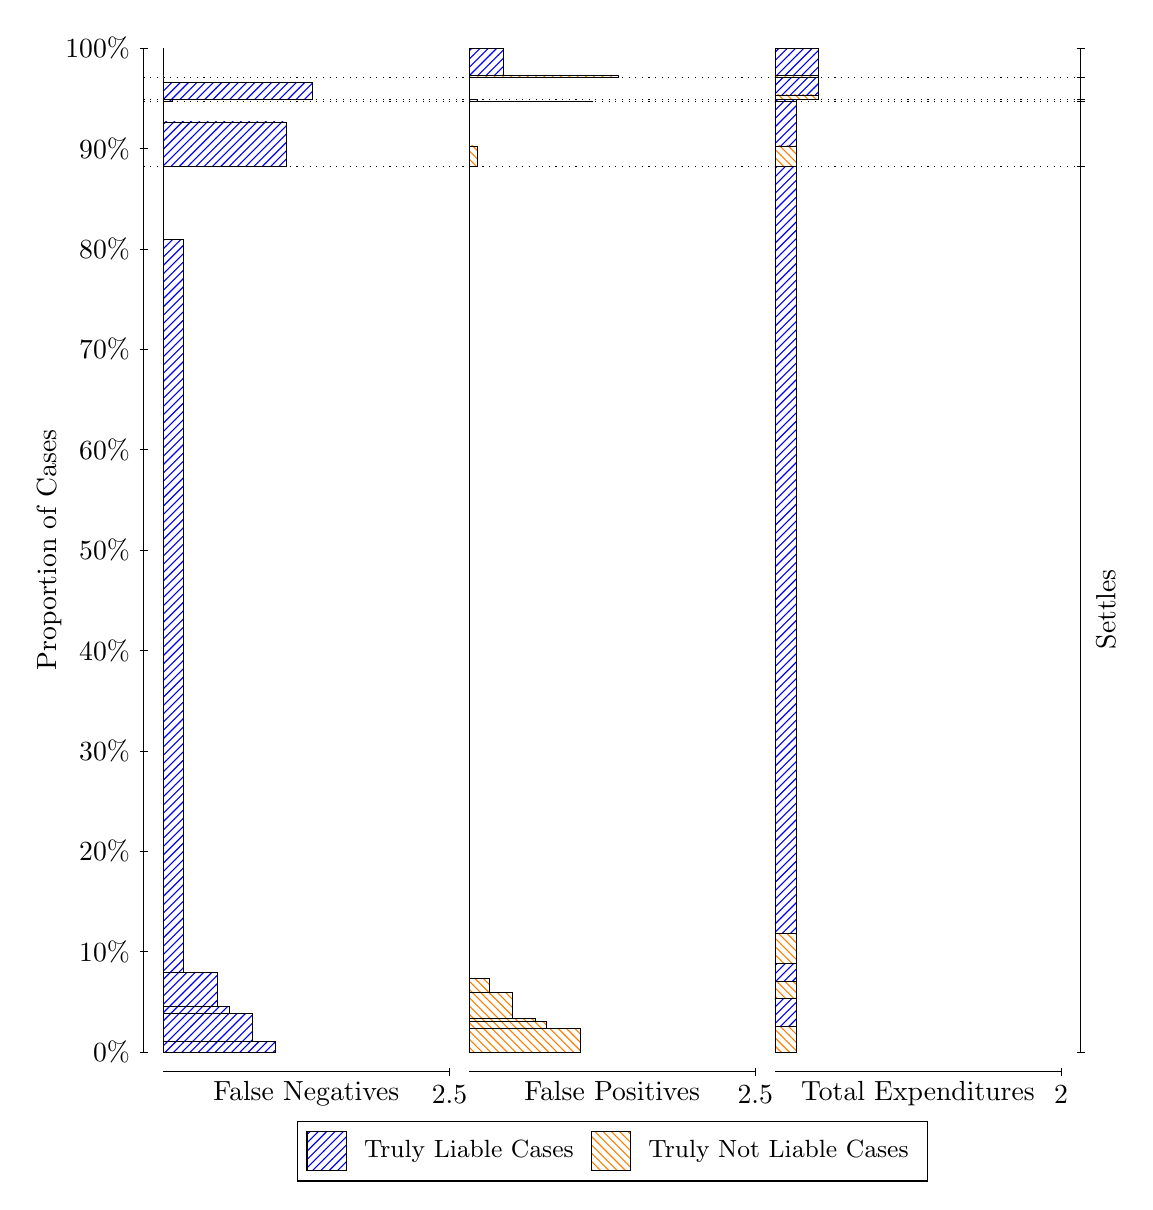
\begin{tikzpicture}
\draw[black, very thin] (1.5,1.75) -- (1.5,14.5);
\node[rotate=90, text=black, anchor=center] at (0.3, 8.125) {Proportion of Cases};
\draw[black, very thin] (1.45,1.75) -- (1.55,1.75);
\node[text=black, anchor=east] at (1.45, 1.75) {0\%};
\draw[black, very thin] (1.45,3.025) -- (1.55,3.025);
\node[text=black, anchor=east] at (1.45, 3.025) {10\%};
\draw[black, very thin] (1.45,4.3) -- (1.55,4.3);
\node[text=black, anchor=east] at (1.45, 4.3) {20\%};
\draw[black, very thin] (1.45,5.575) -- (1.55,5.575);
\node[text=black, anchor=east] at (1.45, 5.575) {30\%};
\draw[black, very thin] (1.45,6.85) -- (1.55,6.85);
\node[text=black, anchor=east] at (1.45, 6.85) {40\%};
\draw[black, very thin] (1.45,8.125) -- (1.55,8.125);
\node[text=black, anchor=east] at (1.45, 8.125) {50\%};
\draw[black, very thin] (1.45,9.4) -- (1.55,9.4);
\node[text=black, anchor=east] at (1.45, 9.4) {60\%};
\draw[black, very thin] (1.45,10.675) -- (1.55,10.675);
\node[text=black, anchor=east] at (1.45, 10.675) {70\%};
\draw[black, very thin] (1.45,11.95) -- (1.55,11.95);
\node[text=black, anchor=east] at (1.45, 11.95) {80\%};
\draw[black, very thin] (1.45,13.225) -- (1.55,13.225);
\node[text=black, anchor=east] at (1.45, 13.225) {90\%};
\draw[black, very thin] (1.45,14.5) -- (1.55,14.5);
\node[text=black, anchor=east] at (1.45, 14.5) {100\%};

\draw[black, very thin] (13.4,1.75) -- (13.4,14.5);
\draw[black, very thin] (13.35,1.75) -- (13.45,1.75);
\node[anchor=west] at (13.35, 1.75) {};
\draw[black, very thin] (13.35,12.997) -- (13.45,12.997);
\node[anchor=west] at (13.35, 12.997) {};
\draw[black, very thin] (13.35,13.821) -- (13.45,13.821);
\node[anchor=west] at (13.35, 13.821) {};
\draw[black, very thin] (13.35,13.845) -- (13.45,13.845);
\node[anchor=west] at (13.35, 13.845) {};
\draw[black, very thin] (13.35,14.125) -- (13.45,14.125);
\node[anchor=west] at (13.35, 14.125) {};
\draw[black, very thin] (13.35,14.5) -- (13.45,14.5);
\node[anchor=west] at (13.35, 14.5) {};

\draw[black, very thin, pattern color=blue, pattern=north east lines] (1.75,1.75) rectangle (3.167,1.8871);
\draw[black, very thin, pattern color=blue, pattern=north east lines] (1.75,1.8871) rectangle (2.8763,2.2431);
\draw[black, very thin, pattern color=blue, pattern=north east lines] (1.75,2.2431) rectangle (2.5857,2.3306);
\draw[black, very thin, pattern color=blue, pattern=north east lines] (1.75,2.3306) rectangle (2.4403,2.7616);
\draw[black, very thin, pattern color=blue, pattern=north east lines] (1.75,2.7616) rectangle (2.0043,12.067);
\draw[black, very thin, pattern color=orange, pattern=north west lines] (1.75,12.067) rectangle (1.75,12.997);
\draw[black, very thin, pattern color=blue, pattern=north east lines] (1.75,12.997) rectangle (3.3123,13.562);
\draw[black, very thin, pattern color=orange, pattern=north west lines] (1.75,13.562) rectangle (1.75,13.821);
\draw[black, very thin, pattern color=blue, pattern=north east lines] (1.75,13.821) rectangle (1.859,13.844);
\draw[black, very thin, pattern color=orange, pattern=north west lines] (1.75,13.844) rectangle (1.75,13.845);
\draw[black, very thin, pattern color=blue, pattern=north east lines] (1.75,13.845) rectangle (3.6393,14.065);
\draw[black, very thin, pattern color=orange, pattern=north west lines] (1.75,14.065) rectangle (1.75,14.125);
\draw[black, very thin, pattern color=orange, pattern=north west lines] (1.75,14.125) rectangle (1.75,14.15);
\draw[black, very thin, pattern color=blue, pattern=north east lines] (1.75,14.15) rectangle (1.75,14.5);
\draw[black, very thin, pattern color=orange, pattern=north west lines] (5.6333,1.75) rectangle (7.0503,2.0473);
\draw[black, very thin, pattern color=orange, pattern=north west lines] (5.6333,2.0473) rectangle (6.6143,2.1395);
\draw[black, very thin, pattern color=orange, pattern=north west lines] (5.6333,2.1395) rectangle (6.469,2.1752);
\draw[black, very thin, pattern color=orange, pattern=north west lines] (5.6333,2.1752) rectangle (6.1783,2.5035);
\draw[black, very thin, pattern color=orange, pattern=north west lines] (5.6333,2.5035) rectangle (5.8877,2.6801);
\draw[black, very thin, pattern color=blue, pattern=north east lines] (5.6333,2.6801) rectangle (5.6333,12.997);
\draw[black, very thin, pattern color=orange, pattern=north west lines] (5.6333,12.997) rectangle (5.7423,13.256);
\draw[black, very thin, pattern color=blue, pattern=north east lines] (5.6333,13.256) rectangle (5.6333,13.821);
\draw[black, very thin, pattern color=orange, pattern=north west lines] (5.6333,13.821) rectangle (7.1957,13.822);
\draw[black, very thin, pattern color=blue, pattern=north east lines] (5.6333,13.822) rectangle (5.7423,13.845);
\draw[black, very thin, pattern color=orange, pattern=north west lines] (5.6333,13.845) rectangle (5.6333,13.905);
\draw[black, very thin, pattern color=blue, pattern=north east lines] (5.6333,13.905) rectangle (5.6333,14.125);
\draw[black, very thin, pattern color=orange, pattern=north west lines] (5.6333,14.125) rectangle (7.5227,14.15);
\draw[black, very thin, pattern color=blue, pattern=north east lines] (5.6333,14.15) rectangle (6.0693,14.5);
\draw[black, very thin, pattern color=orange, pattern=north west lines] (9.5167,1.75) rectangle (9.7892,2.0783);
\draw[black, very thin, pattern color=blue, pattern=north east lines] (9.5167,2.0783) rectangle (9.7892,2.4343);
\draw[black, very thin, pattern color=orange, pattern=north west lines] (9.5167,2.4343) rectangle (9.7892,2.6466);
\draw[black, very thin, pattern color=blue, pattern=north east lines] (9.5167,2.6466) rectangle (9.7892,2.8712);
\draw[black, very thin, pattern color=orange, pattern=north west lines] (9.5167,2.8712) rectangle (9.7892,3.2607);
\draw[black, very thin, pattern color=blue, pattern=north east lines] (9.5167,3.2607) rectangle (9.7892,12.997);
\draw[black, very thin, pattern color=orange, pattern=north west lines] (9.5167,12.997) rectangle (9.7892,13.256);
\draw[black, very thin, pattern color=blue, pattern=north east lines] (9.5167,13.256) rectangle (9.7892,13.821);
\draw[black, very thin, pattern color=orange, pattern=north west lines] (9.5167,13.821) rectangle (9.7892,13.822);
\draw[black, very thin, pattern color=blue, pattern=north east lines] (9.5167,13.822) rectangle (9.7892,13.845);
\draw[black, very thin, pattern color=orange, pattern=north west lines] (9.5167,13.845) rectangle (10.062,13.905);
\draw[black, very thin, pattern color=blue, pattern=north east lines] (9.5167,13.905) rectangle (10.062,14.125);
\draw[black, very thin, pattern color=orange, pattern=north west lines] (9.5167,14.125) rectangle (10.062,14.15);
\draw[black, very thin, pattern color=blue, pattern=north east lines] (9.5167,14.15) rectangle (10.062,14.5);
\draw[black, dotted] (1.5,12.997) -- (13.4,12.997);
\draw[black, dotted] (1.5,13.821) -- (13.4,13.821);
\draw[black, dotted] (1.5,13.845) -- (13.4,13.845);
\draw[black, dotted] (1.5,14.125) -- (13.4,14.125);
\draw[black, very thin] (1.75,1.5) -- (5.3833,1.5);
\node[text=black, anchor=north] at (3.5667, 1.5) {False Negatives};
\draw[black, very thin] (5.3833,1.45) -- (5.3833,1.55);
\node[text=black, anchor=north] at (5.3833, 1.45) {2.5};

\draw[black, very thin] (5.6333,1.5) -- (9.2667,1.5);
\node[text=black, anchor=north] at (7.45, 1.5) {False Positives};
\draw[black, very thin] (9.2667,1.45) -- (9.2667,1.55);
\node[text=black, anchor=north] at (9.2667, 1.45) {2.5};

\draw[black, very thin] (9.5167,1.5) -- (13.15,1.5);
\node[text=black, anchor=north] at (11.333, 1.5) {Total Expenditures};
\draw[black, very thin] (13.15,1.45) -- (13.15,1.55);
\node[text=black, anchor=north] at (13.15, 1.45) {2};

\node[text=black, centered, rotate=90] at (13.72, 7.3733) {Settles};





\draw (7.449999999999999,1.5) node[draw=none] (baseCoordinate) {};
\begin{scope}[align=center]
        \matrix[scale=0.5, draw=black, below=0.5cm of baseCoordinate, nodes={draw}, column sep=0.1cm]{
            \node[rectangle, draw, minimum width=0.5cm, minimum height=0.5cm, pattern color=blue, pattern=north east lines] {}; &
            \node[draw=none, font=\small, text=black] (B) {Truly Liable Cases}; &
            \node[rectangle, draw, minimum width=0.5cm, minimum height=0.5cm, pattern color=orange, pattern=north west lines] {}; &
            \node[draw=none, font=\small, text=black] (B) {Truly Not Liable Cases}; \\
            };
\end{scope}

\end{tikzpicture}
\end{document}